\documentclass[a4paper]{article}

\def\npart {II}
\def\nterm {Michaelmas}
\def\nyear {2015}
\def\nlecturer {C. Birkar}
\def\ncourse {Galois Theory}
\def\nlectures {TTS.12}
\def\nnotready {}

% Imports
\ifx \nextra \undefined
  \usepackage[pdftex,
    hidelinks,
    pdfauthor={Dexter Chua},
    pdfsubject={Cambridge Maths Notes: Part \npart\ - \ncourse},
    pdftitle={Part \npart\ - \ncourse},
  pdfkeywords={Cambridge Mathematics Maths Math \npart\ \nterm\ \nyear\ \ncourse}]{hyperref}
  \title{Part \npart\ - \ncourse}
\else
  \usepackage[pdftex,
    hidelinks,
    pdfauthor={Dexter Chua},
    pdfsubject={Cambridge Maths Notes: Part \npart\ - \ncourse\ (\nextra)},
    pdftitle={Part \npart\ - \ncourse\ (\nextra)},
  pdfkeywords={Cambridge Mathematics Maths Math \npart\ \nterm\ \nyear\ \ncourse\ \nextra}]{hyperref}

  \title{Part \npart\ - \ncourse \\ {\Large \nextra}}
\fi

\author{Lectured by \nlecturer \\\small Notes taken by Dexter Chua}
\date{\nterm\ \nyear}

\usepackage{alltt}
\usepackage{amsfonts}
\usepackage{amsmath}
\usepackage{amssymb}
\usepackage{amsthm}
\usepackage{booktabs}
\usepackage{caption}
\usepackage{enumitem}
\usepackage{fancyhdr}
\usepackage{graphicx}
\usepackage{mathtools}
\usepackage{microtype}
\usepackage{multirow}
\usepackage{pdflscape}
\usepackage{pgfplots}
\usepackage{siunitx}
\usepackage{tabularx}
\usepackage{tikz}
\usepackage{tkz-euclide}
\usepackage[normalem]{ulem}
\usepackage[all]{xy}

\pgfplotsset{compat=1.12}

\pagestyle{fancyplain}
\lhead{\emph{\nouppercase{\leftmark}}}
\ifx \nextra \undefined
  \rhead{
    \ifnum\thepage=1
    \else
      \npart\ \ncourse
    \fi}
\else
  \rhead{
    \ifnum\thepage=1
    \else
      \npart\ \ncourse\ (\nextra)
    \fi}
\fi
\usetikzlibrary{arrows}
\usetikzlibrary{decorations.markings}
\usetikzlibrary{decorations.pathmorphing}
\usetikzlibrary{positioning}
\usetikzlibrary{fadings}
\usetikzlibrary{intersections}
\usetikzlibrary{cd}

\newcommand*{\Cdot}{\raisebox{-0.25ex}{\scalebox{1.5}{$\cdot$}}}
\newcommand {\pd}[2][ ]{
  \ifx #1 { }
    \frac{\partial}{\partial #2}
  \else
    \frac{\partial^{#1}}{\partial #2^{#1}}
  \fi
}

% Theorems
\theoremstyle{definition}
\newtheorem*{aim}{Aim}
\newtheorem*{axiom}{Axiom}
\newtheorem*{claim}{Claim}
\newtheorem*{cor}{Corollary}
\newtheorem*{defi}{Definition}
\newtheorem*{eg}{Example}
\newtheorem*{fact}{Fact}
\newtheorem*{law}{Law}
\newtheorem*{lemma}{Lemma}
\newtheorem*{notation}{Notation}
\newtheorem*{prop}{Proposition}
\newtheorem*{thm}{Theorem}

\renewcommand{\labelitemi}{--}
\renewcommand{\labelitemii}{$\circ$}
\renewcommand{\labelenumi}{(\roman{*})}

\let\stdsection\section
\renewcommand\section{\newpage\stdsection}

% Strike through
\def\st{\bgroup \ULdepth=-.55ex \ULset}

% Maths symbols
\newcommand{\bra}{\langle}
\newcommand{\ket}{\rangle}

\newcommand{\N}{\mathbb{N}}
\newcommand{\Z}{\mathbb{Z}}
\newcommand{\Q}{\mathbb{Q}}
\renewcommand{\H}{\mathbb{H}}
\newcommand{\R}{\mathbb{R}}
\newcommand{\C}{\mathbb{C}}
\newcommand{\Prob}{\mathbb{P}}
\renewcommand{\P}{\mathbb{P}}
\newcommand{\E}{\mathbb{E}}
\newcommand{\F}{\mathbb{F}}
\newcommand{\cU}{\mathcal{U}}
\newcommand{\RP}{\mathbb{RP}}
\newcommand{\CP}{\mathbb{CP}}

\newcommand{\ph}{\,\cdot\,}

\DeclareMathOperator{\sech}{sech}
\DeclareMathOperator{\cosech}{cosech}
\DeclareMathOperator{\cosec}{cosec}

\DeclareMathOperator{\covol}{covol}
\DeclareMathOperator{\vol}{vol}

\let\Im\relax
\let\Re\relax
\DeclareMathOperator{\Im}{Im}
\DeclareMathOperator{\Re}{Re}
\DeclareMathOperator{\im}{im}
\DeclareMathOperator{\image}{image}
\DeclareMathOperator{\Ann}{Ann}

\DeclareMathOperator*{\res}{res}
\DeclareMathOperator{\Res}{Res}
\DeclareMathOperator{\Ind}{Ind}

\DeclareMathOperator{\tr}{tr}
\DeclareMathOperator{\diag}{diag}
\DeclareMathOperator{\rank}{rank}
\DeclareMathOperator{\card}{card}
\DeclareMathOperator{\spn}{span}
\DeclareMathOperator{\adj}{adj}

\DeclareMathOperator{\erf}{erf}
\DeclareMathOperator{\erfc}{erfc}

\DeclareMathOperator{\ord}{ord}
\DeclareMathOperator{\Sym}{Sym}

\DeclareMathOperator{\sgn}{sgn}
\DeclareMathOperator{\orb}{orb}
\DeclareMathOperator{\stab}{stab}
\DeclareMathOperator{\ccl}{ccl}

\DeclareMathOperator{\lcm}{lcm}
\DeclareMathOperator{\hcf}{hcf}

\DeclareMathOperator{\Int}{Int}
\DeclareMathOperator{\id}{id}

\DeclareMathOperator{\betaD}{beta}
\DeclareMathOperator{\gammaD}{gamma}
\DeclareMathOperator{\Poisson}{Poisson}
\DeclareMathOperator{\binomial}{binomial}
\DeclareMathOperator{\multinomial}{multinomial}
\DeclareMathOperator{\Bernoulli}{Bernoulli}
\DeclareMathOperator{\like}{like}

\DeclareMathOperator{\var}{var}
\DeclareMathOperator{\cov}{cov}
\DeclareMathOperator{\bias}{bias}
\DeclareMathOperator{\mse}{mse}
\DeclareMathOperator{\corr}{corr}

\DeclareMathOperator{\otp}{otp}
\DeclareMathOperator{\dom}{dom}

\DeclareMathOperator{\Root}{Root}
\DeclareMathOperator{\supp}{supp}
\DeclareMathOperator{\rel}{rel}
\DeclareMathOperator{\Hom}{Hom}
\DeclareMathOperator{\Aut}{Aut}
\DeclareMathOperator{\Gal}{Gal}
\DeclareMathOperator{\Mat}{Mat}
\DeclareMathOperator{\End}{End}
\DeclareMathOperator{\Char}{char}
\DeclareMathOperator{\ev}{ev}
\DeclareMathOperator{\St}{St}
\DeclareMathOperator{\Lk}{Lk}
\DeclareMathOperator{\disc}{disc}
\DeclareMathOperator{\Isom}{Isom}
\DeclareMathOperator{\length}{length}
\DeclareMathOperator{\energy}{energy}
\DeclareMathOperator{\area}{area}
\DeclareMathOperator{\Syl}{Syl}
\DeclareMathOperator{\cl}{cl}
\DeclareMathOperator{\fix}{fix}

\newcommand{\GL}{\mathrm{GL}}
\newcommand{\SL}{\mathrm{SL}}
\newcommand{\PGL}{\mathrm{PGL}}
\newcommand{\PSL}{\mathrm{PSL}}
\newcommand{\PSU}{\mathrm{PSU}}
\newcommand{\Or}{\mathrm{O}}
\newcommand{\SO}{\mathrm{SO}}
\newcommand{\U}{\mathrm{U}}
\newcommand{\SU}{\mathrm{SU}}

\renewcommand{\d}{\mathrm{d}}
\newcommand{\D}{\mathrm{D}}

\tikzset{->/.style = {decoration={markings,
                                  mark=at position 1 with {\arrow[scale=2]{latex'}}},
                      postaction={decorate}}}
\tikzset{<-/.style = {decoration={markings,
                                  mark=at position 0 with {\arrowreversed[scale=2]{latex'}}},
                      postaction={decorate}}}
\tikzset{<->/.style = {decoration={markings,
                                   mark=at position 0 with {\arrowreversed[scale=2]{latex'}},
                                   mark=at position 1 with {\arrow[scale=2]{latex'}}},
                       postaction={decorate}}}
\tikzset{->-/.style = {decoration={markings,
                                   mark=at position #1 with {\arrow[scale=2]{latex'}}},
                       postaction={decorate}}}
\tikzset{-<-/.style = {decoration={markings,
                                   mark=at position #1 with {\arrowreversed[scale=2]{latex'}}},
                       postaction={decorate}}}

\tikzset{circ/.style = {fill, circle, inner sep = 0, minimum size = 3}}
\tikzset{mstate/.style={circle, draw, blue, text=black, minimum width=0.7cm}}

\definecolor{mblue}{rgb}{0.2, 0.3, 0.8}
\definecolor{morange}{rgb}{1, 0.5, 0}
\definecolor{mgreen}{rgb}{0.1, 0.4, 0.2}
\definecolor{mred}{rgb}{0.5, 0, 0}

\def\drawcirculararc(#1,#2)(#3,#4)(#5,#6){%
    \pgfmathsetmacro\cA{(#1*#1+#2*#2-#3*#3-#4*#4)/2}%
    \pgfmathsetmacro\cB{(#1*#1+#2*#2-#5*#5-#6*#6)/2}%
    \pgfmathsetmacro\cy{(\cB*(#1-#3)-\cA*(#1-#5))/%
                        ((#2-#6)*(#1-#3)-(#2-#4)*(#1-#5))}%
    \pgfmathsetmacro\cx{(\cA-\cy*(#2-#4))/(#1-#3)}%
    \pgfmathsetmacro\cr{sqrt((#1-\cx)*(#1-\cx)+(#2-\cy)*(#2-\cy))}%
    \pgfmathsetmacro\cA{atan2(#2-\cy,#1-\cx)}%
    \pgfmathsetmacro\cB{atan2(#6-\cy,#5-\cx)}%
    \pgfmathparse{\cB<\cA}%
    \ifnum\pgfmathresult=1
        \pgfmathsetmacro\cB{\cB+360}%
    \fi
    \draw (#1,#2) arc (\cA:\cB:\cr);%
}
\newcommand\getCoord[3]{\newdimen{#1}\newdimen{#2}\pgfextractx{#1}{\pgfpointanchor{#3}{center}}\pgfextracty{#2}{\pgfpointanchor{#3}{center}}}

\def\Xint#1{\mathchoice
   {\XXint\displaystyle\textstyle{#1}}%
   {\XXint\textstyle\scriptstyle{#1}}%
   {\XXint\scriptstyle\scriptscriptstyle{#1}}%
   {\XXint\scriptscriptstyle\scriptscriptstyle{#1}}%
   \!\int}
\def\XXint#1#2#3{{\setbox0=\hbox{$#1{#2#3}{\int}$}
     \vcenter{\hbox{$#2#3$}}\kern-.5\wd0}}
\def\ddashint{\Xint=}
\def\dashint{\Xint-}


\begin{document}
\maketitle
{\small
\noindent Field extensions, tower law, algebraic extensions; irreducible polynomials and relation with simple algebraic extensions. Finite multiplicative subgroups of a field are cyclic. Existence and uniqueness of splitting fields.\hspace*{\fill} [6]

\vspace{5pt}
\noindent Existence and uniquness of algebraic closure.\hspace*{\fill} [1]

\vspace{5pt}
\noindent Separability. Theorem of primitive element. Trace and norm.\hspace*{\fill} [3]

\vspace{5pt}
\noindent Normal and Galois extensions, automorphic groups. Fundamental theorem of Galois theory.\hspace*{\fill} [3]

\vspace{5pt}
\noindent Galois theory of finite fields. Reduction mod $p$.\hspace*{\fill} [2]

\vspace{5pt}
\noindent Cyclotomic polynomials, Kummer theory, cyclic extensions. Symmetric functions. Galois theory of cubics and quartics.\hspace*{\fill} [4]

\vspace{5pt}
\noindent Solubility by radicals. Insolubility of general quintic equations and other classical problems.\hspace*{\fill} [3]

\vspace{5pt}
\noindent Artin's theorem on the subfield fixed by a finite group of automorphisms. Polynomial invariants of a finite group; examples.\hspace*{\fill}  [2]}

\tableofcontents

\section{Solving equations}
Here we adopt the notation that if $R$ is a ring, then $R[t]$ is the polynomial ring over $R$ in the variable $t$. Usually, we take $R = \Q$ and consider polynomials $f(t) \in \Q[t]$. The objective is then to find roots to the equation $f(t) = 0$. Often, we want to restrict our search domain. For example, we might ask if there is a root in $\Q$. We will use $\Root_f(X)$ to denote the set of all roots of $f$ in $X$.

We will start from the simple cases, and build up to general solutions of Quartic equations.
\subsection{Linear equations}
Suppose that $f = t + a \in \Q[t]$ (with $a\in \Q$). We have $\Root_f(\Q) = \{-a\}$.

\subsection{Quadratic equations}
Consider a simple quadratic $f = t^2 + 1 \in \Q[t]$. Then $\Root_f(\Q) = \emptyset$ since the square of all rationals are positive. However, in the complex plane, we have $\Root_f(\C) = \{\sqrt{-1}, -\sqrt{-1}\}$.

In general, let $f = t^2 + at + b\in \Q[t]$. Then the roots are given by
\[
  \Root_f(\C) = \left\{\frac{-a \pm \sqrt{a^2 - 4b}}{2}\right\}
\]
\subsection{Cubic equations}
Let $f = t^3 + c\in \Q[t]$. The roots are then
\[
  \Root_f(\C) = \{\sqrt[3]{-c}, \mu\sqrt[3]{-c}, \mu^2 \sqrt[3]{-c}\},
\]
where $\mu = \frac{-1 + \sqrt{-3}}{2}$ is the 3rd root of unity. Note that $\mu$ is defined by the equation $\mu^3 - 1 = 0$, and satisfies $\mu^2 + \mu + 1 = 0$.

In general, let $f = t^3 + at^2 + bt + c \in \Q[t]$, and let $\Root_f(\C) = \{\alpha_1, \alpha_2, \alpha_3\}$, not necessarily distinct.

Our objective is to solve $f = 0$. Before doing so, we have to make it explicit what we mean by ``solving'' the equation. As in solving the quadratic, we want to express the roots $\alpha_1, \alpha_2$ and $\alpha_3$ in terms of ``radicals'' involving $a, b$ and $c$.

Unlike the quadratic case, there is no straightforward means of coming up with a general formula. The result we currently have is the result of many many years of hard work, and the substitutions we make seemingly come out of nowhere. However, after a lot of magic, we will indeed come up with a general formula for it.

We first simplify our polynomial by assuming $a = 0$. Given any polynomial $f = t^3 + at^2 + bt + c$, we can perform the change of variables $t\mapsto t - \frac{a}{3}$, and get rid of the coefficient of $a^2$. So we can assume $a = 0$.

Let $\mu$ be as above. Define
\begin{align*}
  \beta &= \alpha_1 + \mu \alpha_2 + \mu^2 \alpha_3\\
  \gamma &= \alpha_1 + \mu^2 \alpha_2 + \mu \alpha_3
\end{align*}
These are the \emph{Lagrange resolvers}. We obtain
\begin{align*}
  \beta\gamma &= \alpha_1^2 + \alpha_2^2 +\alpha_3^2 + (\mu + \mu^2)(\alpha_1\alpha_2 + \alpha_2\alpha_3 + \alpha_1\alpha_3)\\
  \intertext{Since $\mu^2 + \mu + 1 = 0$, we have $\mu^2 + \mu = -1$. So we can simplify to obtain}
  &= (\alpha_1 + \alpha_2 + \alpha_3)^2 - 3(\alpha_1\alpha_2 + \alpha_2\alpha_3 + \alpha_1\alpha_3)\\
  \intertext{We have $\alpha_1 + \alpha_2 + \alpha_3 = -a = 0$, while $b = \alpha_1\alpha_2 + \alpha_2\alpha_3 + \alpha_1\alpha_3$. So}
  &= -3b\\
  \intertext{Cubing, we obtain}
  \beta^3\gamma^3 &= -27b^3.
\end{align*}
On the other hand, recalling again that $\alpha_1 + \alpha_2 + \alpha_3 = 0$, we have
\begin{align*}
  \beta^3 + \gamma^3 &= (\alpha_1 + \mu \alpha_2 + \mu^2 \alpha_3)^3 + (\alpha_1 + \mu^2\alpha_2 + \mu \alpha_3)^3 + (\alpha_1 + \alpha_2 + \alpha_3)^3\\
  &= 3(\alpha_1^2 + \alpha_2^3 + \alpha_3^2) + 18\alpha_1\alpha_2\alpha_3\\
  \intertext{We have $\alpha_1\alpha_2\alpha_3 = -c$, and since $\alpha_i^3 + b\alpha_i + c = 0$ for all $i$, summing gives $\alpha_1^3 +  \alpha_2^3 + \alpha_3^3 + 3c = 0$. So}
  &= -27c
\end{align*}
Hence, we obtain
\[
  (t - \beta^3)(t - \gamma^3) = t^2 + 27ct - 27b^3.
\]
We already know how to solve this equation using the quadratic formula. We obtain
\[
  \{\beta^3, \gamma^3\} = \left\{\frac{-27 c \pm \sqrt{(27c)^3 + 4\times 27b^3}}{2}\right\}
\]
We now have $\beta^3$ and $\gamma^3$ in terms of radicals. So we can find $\beta$ and $\gamma$ in terms of radicals. Finally, we can solve for $\alpha_i$ using
\begin{align*}
  0 &= \alpha_1 + \alpha_2 + \alpha_3\\
  \beta &= \alpha_1 + \mu \alpha_2 + \mu^2 \alpha_3\\
  \gamma &= \alpha_1 + \mu^2 \alpha_2 + \mu \alpha_3
\end{align*}
In particular, we obtain
\begin{align*}
  \alpha_1 &= \frac{1}{3}(\beta + \gamma)\\
  \alpha_2 &= \frac{1}{3}(\mu^2 \beta + \mu \gamma)\\
  \alpha_3 &= \frac{1}{3}(\mu \beta + \mu^2 \gamma)
\end{align*}
So we can solve a cubic in terms of radicals.

This was a lot of magic involved, and indeed this was discovered through a lot of hard work throughout many many years. This is also not a very helpful result since we have no idea where these substitutions came from and why they intuitively work.

\subsection{Quartic equations}
Assume $f = t^4 + at^3 + bt^2 + ct + d\in \Q[t]$. Let $\Root_f(\C) = \{\alpha_1, \alpha_2, \alpha_3, \alpha_4\}$. Can we express all these in terms of radicals? Again the answer is yes, but the procedure is much more complicated.

We can perform a similar change of variable to assume $a = 0$. So $\alpha_1 + \alpha_2 + \alpha_3 + \alpha_4 = 0$.

This time, define
\begin{align*}
  \beta &= \alpha_1 + \alpha_2\\
  \gamma &= \alpha_1 + \alpha_3\\
  \lambda &= \alpha_1 + \alpha_4
\end{align*}
Doing some calculations, we see that
\begin{align*}
  \beta^2 &= -(\alpha_1 + \alpha_2)(\alpha_3 + \alpha_4)\\
  \gamma^2 &= -(\alpha_1 + \alpha_3)(\alpha_2 + \alpha_4)\\
  \lambda^2 &= -(\alpha_1 + \alpha_4)(\alpha_2 + \alpha_3)
\end{align*}
Now consider
\begin{align*}
  g &= (t - \beta^2)(t - \gamma^2)(t - \lambda^2)\\
  &= t^3 + 2bt^2 + (b^2 - 4d)t - c^2
\end{align*}
This we know how to solve, and so we are done.

\subsection{Quintics and above}
So far so good. But how about polynomials of higher degrees? In general, let $f \in \Q[t]$. Can we write down all the roots of $f$ in terms of radicals? We know that the answer is yes if $\deg f \leq 4$.

Unfortunately, for $\deg f \geq 5$, the answer is no. Of course, this ``no'' means no \emph{in general}. For example, $f = (t - 1)(t - 2) \cdots (t - 5)\in \Q[t]$ has the obvious roots in terms of radicals.

There isn't an easy proof of this result. We will first have to associate a \emph{field extension} $F \supseteq \Q$ for our polynomial $f$. Then we associate a \emph{Galois group} $G$ to this field extension. We will show that $f$ has a solution in terms of radicals iff the Galois group is ``soluble'', where ``soluble'' has a specific algebraic definition in group theory we will explore later. This process is what we will study in Galois theory.

In a nutshell, Galois theory is the study of field extensions and the associated Galois groups. Nowadays, Galois theory finds its applications in number theory, algebraic geometry and even cryptography.

\section{Field extensions}
After all that (hopefully) fun introduction and motivation, we will now start Galois theory in a more abstract way. Everything starts from field extensions.

\begin{defi}[Field extension]
  A \emph{field extension} is an inclusion of a field $E\subseteq F$, where $E$ inherits the algebraic operations from $F$. Alternatively, we can define this by a injective homomorphism $E\to F$. We say $F$ is an \emph{extension} of $E$, and $E$ is a \emph{subfield} of $F$.
\end{defi}

\begin{eg}\leavevmode
  \begin{enumerate}
    \item $\Q\subseteq \R$ is a field extension.
    \item $\Q \subseteq \C$ is a field extension.
    \item $\Q\subseteq \Q(\sqrt{2}) = \{a + b\sqrt{2}: a, b\in \Q\} \subseteq \R$ is a field extension.
  \end{enumerate}
\end{eg}

Now suppose $K\subseteq L$ is a field extension. We can consider $L$ as a vector space over $K$. We know that $L$ already comes with an additive abelian group structure, and we can define scalar multiplication by simply multiplying: if $a\in K, \alpha\in L$, then $a\cdot \alpha$ is simply defined as multiplication in $L$.

\begin{defi}[Degree of field extension]
  The \emph{degree} of $L$ over $K$ is $[L:K]$ is the dimension of $L$ as a vector space over $K$. The extension is \emph{finite} if the degree is finite.
\end{defi}
In this course, we are mostly concerned with finite extensions.

\begin{eg}\leavevmode
  \begin{enumerate}
    \item Consider $\R\subseteq \C$. This is a finite extension with degree $[\C:\R] = 2$ since we have a basis of $\{1, i\}$.
    \item The extension $\Q\subseteq \Q(\sqrt{2})$ has degree $2$ since we have a basis of $\{1, \sqrt{2}\}$.
    \item The extension $\Q\subseteq \R$ is not finite.
  \end{enumerate}
\end{eg}

\begin{thm}[Tower Law]
  Let $K\subseteq L \subseteq F$ be field extensions. Then
  \[
    [F:K] = [F:L][L:K]
  \]
\end{thm}

\begin{proof}
  Assume $[F:L]$ and $[L:K]$ are finite. Let $\{\alpha_1, \cdots, \alpha_m\}$ be a basis for $L$ over $K$, and $\{\beta_1, \cdots, \beta_n\}$ be a basis for $F$ over $L$. Pick $\gamma \in F$. Then we can write
  \[
    \gamma = \sum_i b_i \beta_i,\quad b_i\in L.
  \]
  For each $b_i$, we can write as
  \[
    b_i = \sum_j a_{ij}\alpha_{j},\quad a_{ij}\in K.
  \]
  So we can write
  \[
    \gamma = \sum_i \left(\sum_j a_{ij}\alpha_j\right)\beta_i = \sum_{i, j} a_{ij}\alpha_j \beta_i.
  \]
  So $T = \{\alpha_j\beta_i\}_{i, j}$ spans $F$ over $K$. To show that this is a basis, we have to show that they are linearly independent. Consider the case where $\gamma = 0$. Then we must have $b_i = 0$ since $\{\beta_i\}$ is a basis of $F$ over $L$. Hence each $a_{ij} = 0$ since $\{\alpha_j\}$ is a basis of $L$ over $K$.

  This implies that $T$ is a basis of $F$ over $K$. So
  \[
    [F:K] = |T| = nm = [F:L][L:K].
  \]
  Finally, if $[F:L] = \infty$ or $[L:K] = \infty$, then clearly $[F:K] = \infty$ as well. So equality holds as well.
\end{proof}

\begin{defi}[Algebraic number]
  Let $K\subseteq L$ be a field extension, $\alpha\in L$. We define
  \[
    I_\alpha = \{f\in K[t] : f(\alpha) = 0\}\subseteq K[t]
  \]
  This is the set of polynomials for which $\alpha$ is a root. It is easy to show that $I_\alpha$ is an ideal, since it is the kernel of the ring homomorphism $K[t] \to L$ by $g \mapsto g(\alpha)$.

  We say $\alpha$ is \emph{algebraic} over $K$ if $I_\alpha \not= 0$. Otherwise, $\alpha$ is \emph{transcendental} over $K$.

  We say $L$ is \emph{algebraic} over $K$ if every element of $L$ is algebraic.
\end{defi}

\begin{eg}\leavevmode
  \begin{enumerate}
    \item $\sqrt[9]{7}$ is algebraic over $\Q$ because $f(\sqrt[9]{7}) = 0$, where $f = t^9 - 7$. In general, any number written with radicals is algebraic over $\Q$.
    \item $\pi$ is not algebraic over $\Q$.
  \end{enumerate}
\end{eg}
These are rather simple examples, and the following lemma will provide us a way of generating much more examples.

\begin{lemma}
  Let $K\subseteq L$ be a finite extension. Then $L$ is algebraic over $K$.
\end{lemma}

\begin{proof}
  Let $n = [L:K]$, and let $\alpha\in L$. Then $1, \alpha, \alpha^2, \cdots, \alpha^n$ are linearly dependent over $K$ (since there are $n + 1$ elements). So there exists some $a_i \in K$ (not all zero) such that
  \[
    a_n \alpha^n + a_{n - 1}\alpha^{n - 1} + \cdots + a_1 \alpha + a_0 = 0.
  \]
  So we have a non-trivial polynomial that vanishes at $\alpha$. So $\alpha$ is algebraic over $K$.

  Since $\alpha$ was arbitrary, $L$ itself is algebraic.
\end{proof}

Let $K\subseteq L$ be a field extension, $\alpha\in L$ algebraic. Since $K$ is a field, $K[t]$ is a PID (principal ideal domain). So $I_\alpha = \bra P_\alpha\ket$ for some monic $P_\alpha \in K[t]$. So every element of $I_\alpha$ is just a multiple of $P_\alpha$.
\begin{defi}[Minimal polynomial]
  Let $K\subseteq L$ be a field extension, $\alpha \in L$. The \emph{minimal polynomial} of $\alpha$ over $K$ is a monic polynomial $P_\alpha$ such that $I_\alpha = \bra P_\alpha\ket$.
\end{defi}

\begin{eg}\leavevmode
  \begin{enumerate}
    \item Consider $\Q\subseteq\R$, $\alpha = \sqrt[3]{2}$. Then the minimal polynomial is $P_\alpha = t^3 - 2$.
    \item Consider $\R\subseteq\C$, $\alpha = \sqrt[3]{2}$. Then the minimal polynomial is $P_\alpha = t - \sqrt[3]{2}$.
  \end{enumerate}
\end{eg}
\begin{prop}
  Let $K\subseteq L$ be a field extension, $\alpha\in L$ algebraic over $K$, and $P_\alpha$ the minimal polynomial. Then $P_\alpha$ is irreducible in $K[t]$.
\end{prop}

\begin{proof}
  Assume that $P_\alpha = QR$ in $K[t]$. So $0 = P_\alpha(\alpha) = Q(\alpha) R(\alpha)$. So $Q(\alpha) = 0$ or $R(\alpha) = 0$. Say $Q(\alpha) = 0$. So $Q\in I_\alpha$. So $Q$ is a multiple of $P_\alpha$. However, we also know that $P_\alpha$ is a multiple of $Q_\alpha$. This is possible only if $R$ is a unit in $K[t]$, ie. $R\in K$. So $P_\alpha$ is irreducible.
\end{proof}

\begin{defi}[Field generated by $\alpha$]
  Let $K\subseteq L$ be a field extension, $\alpha\in L$. We define $K(\alpha)$ to be the smallest subfield of $L$ containing $K$ and $\alpha$. We call $K(\alpha)$ the \emph{field generated by $\alpha$ over $K$}.
\end{defi}

\begin{thm}
  Let $K\subseteq L$ a field extension, $\alpha\in L$ algebraic. Then
  \begin{enumerate}
    \item $K(\alpha)$ is the image of the (ring) homomorphism $\phi: K[t] \to L$ defined by $f \mapsto f(\alpha)$.
    \item $[K(\alpha): K] = \deg P_\alpha$, where $P_\alpha$ is the minimal polynomial of $\alpha$ over $K$.
  \end{enumerate}
\end{thm}

\begin{proof}\leavevmode
  \begin{enumerate}
    \item Let $F$ be the image of $\phi$. Then $F$ is a subring of $L$ as $F$ is the image of a ring homomorphism. We show that $F$ is a field.

      Suppose $\beta\in F$ is non-zero. We want to find an inverse.

      By definition, $\beta = f(\alpha)$ for some $f\in K[t]$. Since $\beta \not= 0$, $f(\alpha) \not= 0$. So $f \not \in I_\alpha = \bra P_\alpha\ket$. So $P_\alpha \nmid f$ in $K[t]$. Since $P_\alpha$ is irreducible, $P_\alpha$ and $f$ are coprime. Then there exists some $g, h \in K[t]$ such that $fg + hP_\alpha = 1$. So $f(\alpha)g(\alpha) = f(\alpha) g(\alpha) + h(\alpha)P_\alpha(\alpha) = 1$. So $\beta g(\alpha) = 1$. So $\beta$ has an inverse. So $F$ is a field.

      From the definition of $F$, we have $K\subseteq F$ and $\alpha \in F$, using the constant polynomials $f = c \in K$ and the identity $f = t$.

      Now, if $K\subseteq G\subseteq L$ and $\alpha \in G$, then $G$ contains all the polynomial expressions of $\alpha$. Hence $F\subseteq G$. So $K(\alpha) = F$.
    \item Let $n = \deg P_\alpha$. We show that $\{1, \alpha, \alpha^2, \cdots, \alpha^{n - 1}\}$ is a basis for $K(\alpha)$ over $K$.

      First note that since $\deg P_\alpha = n$, we can write
      \[
        \alpha^n = \sum_{i = 0}^{n - 1} a_i \alpha^i.
      \]
      So any other higher powers are also linear combinations of the $\alpha^i$s (by induction). This means that $K(\alpha)$ is spanned by $1, \cdots, \alpha^{n - 1}$ as a $K$ vector space.

      It remains to show that $\{1, \cdots, \alpha^{n - 1}\}$ is linearly independent. Assume not. Then for some $b_i$, we have
      \[
        \sum b_i \alpha^i = 0.
      \]
      Let $f = \sum b_i t^i$. Then $f(\alpha) = 0$. So $f \in I_\alpha = \bra P_\alpha\ket$. However, $\deg f < \deg P_\alpha$. So we must have $f = 0$. So all $b_i = 0$. So $\{1, \cdots, \alpha^{n - 1}\}$ is a basis for $K(\alpha)$ over $K$. So $[K(\alpha): K] = n$.
  \end{enumerate}
\end{proof}

\begin{cor}
  Let $K\subseteq L$ be a field extension, $\alpha \in L$. Then $\alpha$ is algebraic over $K$ if and only if $K \subseteq K(\alpha)$ is a finite extension.
\end{cor}

\begin{proof}
  If $\alpha$ is algebraic, then $[K(\alpha): K] = \deg P_\alpha < \infty$ by above. So the extension is finite.

  If $K\subseteq K(\alpha)$ is a finite extension, then by previous lemma, the entire $K(\alpha)$ is algebraic over $K$. So $\alpha$ is algebraic over $K$.
\end{proof}

We can extend this definition to allow more elements in the generating set.
\begin{defi}[Field generated by elements]
  Let $K\subseteq L$ be a field extension, $\alpha_1, \cdots, \alpha_n\subseteq L$. We define $K(\alpha_1, \cdots, \alpha_n)$ to be the smallest subfield of $L$ containing $K$ and $\alpha_1, \cdots, \alpha_n$.

  We call $K(\alpha_1, \cdots, \alpha_n)$ the \emph{field generated by} $\alpha_1, \cdots, \alpha_n$ over $K$.
\end{defi}

\begin{thm}[]
  Suppose that $K\subseteq L$ is a field extension.
  \begin{enumerate}
    \item If $\alpha_1, \cdots, \alpha_n \in L$ are algebraic over $K$, then $K\subseteq K(\alpha_1, \cdots, \alpha_n)$ is a finite extension.
    \item If we have $K\subseteq F\subseteq L$ and $K\subseteq F$ is a finite extension, then $F = K(\alpha_1, \cdots, \alpha_n)$ for some $\alpha_1,\cdots, \alpha_n \in L$.
  \end{enumerate}
\end{thm}

\begin{proof}\leavevmode
  \begin{enumerate}
    \item We prove this by induction. Since $\alpha_1$ is algebraic over $K$, $K\subseteq K(\alpha_1)$ is a finite extension.

      For $1 \leq i < n$, $\alpha_{i + 1}$ is algebraic over $K$. So $\alpha_{i + 1}$ is also algebraic over $K(\alpha_1, \cdots, \alpha_i)$. So $K(\alpha_1, \cdots, \alpha_i)\subseteq K(\alpha_1, \cdots, \alpha_i)(\alpha_{i + 1})$ is a finite extension. But $K(\alpha_1, \cdots, \alpha_i)(\alpha_{i + 1}) = K(\alpha_1, \cdots, \alpha_{i + 1})$. By the tower law, $K \subseteq K(\alpha_i, \cdots, \alpha_{i + 1})$ is a finite extension.

    \item Since $F$ is a finite dimensional vector space, we can take a basis $\{\alpha_1, \cdots, \alpha_n\}$ of $F$ over $K$. Then it should be clear that $F = K(\alpha_1, \cdots, \alpha_n)$.
  \end{enumerate}
\end{proof}

When studying polynomials, the following result from IB Groups, Rings and Modules is often helpful:
\begin{prop}[Eisenstein's criterion]
  Let $f = a_nt^n + \cdots + a_1 t + a_0\in \Z[t]$. Assume that there is some prime number $p$ such that
  \begin{enumerate}
    \item $ p | a_i$ for all $i < n$.
    \item $p \nmid a_n$
    \item $p^2 \nmid a_0$.
  \end{enumerate}
  Then $f$ is irreducible in $\Q[t]$.
\end{prop}

\begin{eg}
  Consider the field extensions
  \[
    \Q \subseteq \Q(\sqrt{2})\subseteq \Q(\sqrt{2}, \sqrt[3]{2})\subseteq \R,
  \]
  \[
    \Q\subseteq \Q(\sqrt[3]{2}) \subseteq \Q(\sqrt{2}, \sqrt[3]{2})\subseteq \R.
  \]
  We have $[\Q(\sqrt{2}: \Q] = 2$ since $\{1, \sqrt{2}\}$ is a basis of $\Q(\sqrt{2})$ over $\Q$.

  How about $[\Q(\sqrt[3]{2}):\Q]$? By the Eisenstein criterion, we know that $t^3 - 2$ is irreducible in $\Q[t]$. So the minimal polynomial of $\sqrt[3]{2}$ over $\Q$ is $t^3 - 2$ which has dergee 3. So $[\Q(\sqrt[3]{2}):\Q] = 3$.

  These results immediately tells that $\sqrt[3]{2}\not\in \Q(\sqrt{2})$. Otherwise, this entails that $\Q(\sqrt[3]{2}) \subseteq \Q(\sqrt{2})$. Then the power law says that
  \[
    [\Q(\sqrt{2}):\Q] = [\Q(\sqrt{2}):\Q(\sqrt[3]{2})][\Q(\sqrt[3]{2}):\Q].
  \]
  In particular, plugging the numbers in entails that that $3$ is a factor of $2$, which is clearly nonsense. Simiarly, $\sqrt{2}\not \in \Q(\sqrt[3]{2})$.

  How about the inclusion $\Q(\sqrt{2})\subseteq \Q(\sqrt{2}, \sqrt[3]{2})$? We now show that the minimal polynomial $P_{\sqrt[3]{2}}$ of $\sqrt[3]{2}$ over $\Q(\sqrt{2})$ is $t^3 - 2$.

  Suppose not. Then $t^3 - 2$ is reducible, with the real $P_{\sqrt[3]{2}}$ as one of its factors. Let $t^3 - 2 = P_{\sqrt[3]{2}} \cdot R$ for some non-unit polynomial $R$.

  We know that $P_{\sqrt[3]{2}}$ does not have degree 3 (or else it would be $t^3 - 2$), and not degree 1, since a degree 1 polynomial has a root. So it has degree $2$. So $R$ has degree $1$. Then $R$ has a root, ie. $R(\beta) = 0$ for some $\beta \in \Q(\sqrt{2})$. So $\beta^3 - 2 = 0$. Hence $[\Q(\beta): \Q] = 3$.
  \[
    [\Q(\sqrt{2}):\Q] = [\Q(\sqrt{2}):\Q(\beta)][\Q(\beta):\Q].
  \]
  Again, this is nonsense since it entails that 3 is a factor of 2. So the minimal polynomial is indeed $t^3 -2$. So $[\Q(\sqrt{2}, \sqrt[3]{2}):\Q] = 6$ by the tower law.

  Alternatively, we can obtain this result by noting that the tower law on $\Q \subseteq \Q(\sqrt{2})\subseteq \Q(\sqrt{2}, \sqrt[3]{2})$ and $\Q\subseteq \Q(\sqrt[3]{2}) \subseteq \Q(\sqrt{2}, \sqrt[3]{2})$ entails that 2 and 3 are both factors of $[\Q(\sqrt{2}, \sqrt[3]{2}):\Q]$. So it is at least $6$. Then since $t^3 - 2\in \Q(\sqrt{2})[t]$ has $\sqrt[3]{2}$ as a root, the degree is at most 6. So it is indeed 6.
\end{eg}
\section{Some applications of field extensions}
\subsection{Ruler and compass constructions}
We are going to look at some classic problems in geometry, and solve them using field extensions. In particular, we want to show that certain things cannot be constructed using a compass and a ruler (note that we assume that the ruler does not have markings on it).

It is often easy to prove that certain things are constructible - just exhibit an explicit construction of it. However, it is much more difficult to show that things are \emph{not} constructible. Two classical examples are
\begin{enumerate}
  \item Doubling the cube: Given a cube, can we construct the side of another cube whose volume is double the volume of the original cube?
  \item Given an angle, can we divide the angle into three equal angles?
\end{enumerate}
The idea here is to associate with each possible construction a field extension, and then prove certain results about how these field extensions should behave. We then show that if we could, say, double the cube, then this construction would inevitable break some of the properties it should have.

Firstly, we want to formulate our problem in a more convenient way. In particular, we will view the plane as $\R^2$, and describe lines and circles by equations. We also want to describe ``compass and ruler'' constructions in a more solid way.
\begin{defi}[Constructible points]
  Let $S\subseteq \R^2$ be a set of (usually finite) points in the plane.

  A ``ruler'' allows us to do the following: if $P, Q\in S$, then we can draw the line passing through $P$ and $Q$.

  A ``compass'' allows us to do the following: if $P, Q, Q'\in S$, then we can draw the circle with center at $P$ and radius of length $QQ'$.

  Any point $R\in \R^2$ is \emph{1-step constructible} from $S$ if $R$ belongs to the intersection of two distinct lines or circles constructed from $S$ using rulers and compasses.

  A point $R\in \R^2$ is \emph{constructible} from $S$ if there is some $R_1, \cdots, R_n = R \in \R^2$ such that $R_{i + 1}$ is 1-step constructible from $S\cup \{R_1, \cdots, R_i\}$ for each $i$.
\end{defi}

\begin{eg}
  Let $S = \{(0, 0), (1, 0)\}$. What can we construct? It should be easy to see that $(n, 0)$ for all $n \in \Z$ are all constructible from $S$. In fact, we can show that all points of the form $(m, n)\in \Z$ are constructible from $S$.
  \begin{center}
    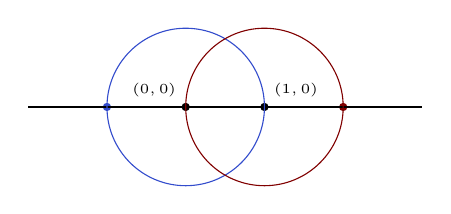
\begin{tikzpicture}
      \node [circ] at (0, 0) {};
      \node [anchor = south east] at (0, 0) {\tiny $(0, 0)$};
      \node [circ] at (1, 0) {};
      \node [anchor = south west] at (1, 0) {\tiny $(1, 0)$};
      \node [mblue] [circ] at (-1, 0) {};
      \node [mred] [circ] at (2, 0) {};

      \draw (-2, 0) -- (3, 0);
      \draw [mblue] circle [radius=1];
      \draw [mred] (1, 0) circle [radius = 1];
    \end{tikzpicture}
  \end{center}
\end{eg}

\begin{defi}[Field of $S$]
  Let $S\subseteq \R^2$ be finite. Define the \emph{field of} $S$ by
  \[
    \Q(S) = \Q(\{\text{coordinates of points in }S\}) \subseteq \R,
  \]
  where we put in the $x$ coordinate and $y$ coordinate separately into the generating set.
\end{defi}
For example, if $S = \{(\sqrt{2}, \sqrt{3})\}$, then $\Q(S) = \Q(\sqrt{2}, \sqrt{3})$.

The key theorem we will use to prove our results is
\begin{thm}[]
  Let $S\subseteq \R^2$ be finite. Then
  \begin{enumerate}
    \item If $R$ is 1-step constructible from $S$, then $[\Q(S\cup \{R\}):\Q(S)] = 1$ or $2$.
    \item If $T\subseteq \R^2$ is finite, $S\subseteq T$, and the points in $T$ are constructible from $S$, Then $[\Q(S\cup T): \Q(S)] = 2^k$ for some $k$ (where $k$ can be $0$).
  \end{enumerate}
\end{thm}

\begin{proof}
  By assumption, there are distinct lines or circles $C, C'$ constructed from $S$ using ruler and compass, such that $R\in C\cap C'$. By elementary geometry, $C$ and $C'$ can be given by the equations
  \begin{align*}
    C&: a(x^2 + y^2) + bx + cy + d = 0,\\
    C'&: a'(x^2 + y^2) + b'x + c'y + d' = 0.
  \end{align*}
  where $a, b, c, d, a', b', c', d' \in \Q(S)$. In particular, if we have a line, then we can take $a = 0$.

  Let $R = (r_1, r_2)$. If $a = a' = 0$ (ie. $C$ and $C'$ are lines), then solving the two linear equations gives $r_1, r_2 \in \Q(S)$. So $[\Q(S\cup \{R\}):\Q(S)] = 1$.

  So we can now assume wlog that $a\not = 0$. We let
  \[
    p = a'b - ab',\quad a'c - ac',\quad \ell = a'd - ad',
  \]
  which are the coefficients when we perform $a'\times C - a \times C'$. Then by assumption, $p \not= 0$ or $q \not= 0$. Otherwise, $c$ and $c'$ would be the same curve. wlog $p \not= 0$. Then since $(r_1, r_2)$ satisfy both equations of $C$ and $C'$, they satisfy
  \[
    px + qy + \ell = 0.
  \]
  In other words, $pr_1 + qr_2 + \ell = 0$. This tells us that
  \[
    r_1 = -\frac{qr_2 + \ell}{p}.\tag{*}
  \]
  If we put $r_1, r_2$ into the equations of $C$ and $C'$ and use $(*)$, we get an equation of the form
  \[
    \alpha r_2^2 + \beta r_2  + \gamma = 0,
  \]
  where $\alpha, \beta, \gamma \in \Q(S)$. So we can find $r_2$ (and hence $r_1$ using linear relations) using only a single radical of degree 2. So
  \[
    [\Q(S\cup \{R\}):\Q(S)] = [\Q(S)(r_2): \Q(S)] = 1\text{ or }2,
  \]
  since the minimal polynomial of $r_2$ over $\Q(S)$ has degree 1 or 2.

  Then (ii) follows directly from induction, using the tower law.
\end{proof}
\begin{cor}
  It is impossible to ``double the cube''.
\end{cor}

\begin{proof}
  Consider the cube with unit side length, ie. we are given the set $S = \{(0, 0), (1, 0)\}$. Then doubling the cube would correspond to constructing a side of length $\ell$ such that $\ell^3 = 2$, ie. $\ell = \sqrt[3]{2}$. Thus we need to construct a point $R = (\sqrt[3]{2}, 0)$ from $S$.

  If we can indeed construct this $R$, then we need
  \[
    [\Q(S\cup \{R\}):\Q(S)] = 2^k
  \]
  for some $k$.  But we know that $\Q(S) = \Q$ and $\Q(S\cup \{R\}) = \Q(\sqrt[3]{2})$, and that
  \[
    [\Q(\sqrt[3]{2}):\Q] = 3.
  \]
  This is a contradiction since $3$ is not a power of $2$.
\end{proof}
\end{document}
